
%%%%%%%%%%%%%%%%%%%%%%%%%%%%%%%%%%%%%%%%%%%%%%%%%%%%%%%%
% LaTex Template for proposals within the              %
% DFG Research Unit Program                            %         
%Planet Formation Witnesses and Probes: Transition Discs
% August 2016                                            %                           
%                                                      %
%%%%%%%%%%%%%%%%%%%%%%%%%%%%%%%%%%%%%%%%%%%%%%%%%%%%%%%%
%
% 
%
% This template may be used to prepare proposals in latex.
%
%
% The project description, including publication list, should be no more than 20 pages
% in length. It should be self-explanatory and not require reviewers to read the 
% literature that is quoted or enclosed.

\documentclass[10pt,fleqn,twoside]{article}

%%%% USE ARIAL FONT %%%%%%%%%%%%%%%%%%%%%%%%%%%%%%%%%%%%%%%%%%%%%%%%%%%%%%
\usepackage{helvet}
\renewcommand\familydefault{phv}

%%%% INCLUDE NECESSARY PACKAGES %%%%%%%%%%%%%%%%%%%%%%%%%%%%%%%%%%%%%%%%%%
%\usepackage{babel}
\usepackage[UKenglish]{babel}
\usepackage{amsmath}
\usepackage{amssymb}
\usepackage{fancyhdr}
\usepackage{natbib}
\usepackage{xcolor}
\usepackage{ae,aecompl}
\usepackage{graphicx}
\usepackage{palatino}
\usepackage[T1]{fontenc}
\usepackage{rotating}
\usepackage{epsf}
\usepackage{setspace}
\usepackage{sfmath}
\usepackage{sidecap}

%%%% PAGE LAYOUT %%%%%%%%%%%%%%%%%%%%%%%%%%%%%%%%%%%%%%%%%%%%%%%%%%%%%%%%%
\setlength{\textheight}{22cm}
\setlength{\topmargin}{-1.2cm}
\setlength{\textwidth}{15.6cm}
\setlength{\oddsidemargin}{0.0cm}
\setlength{\evensidemargin}{0.0cm}
\setlength{\mathindent}{1.5cm}
\setlength{\parindent}{0.0cm}
\setlength{\parskip}{0.08cm}

%%%% PAGE HEADER %%%%%%%%%%%%%%%%%%%%%%%%%%%%%%%%%%%%%%%%%%%%%%%%%%%%%%%%%%
\pagestyle{fancy}
\fancyhead[RE,RO]{}
\fancyfoot[RO]{ \thepage}
\fancyfoot[LE]{ \thepage}
\fancyfoot[CE,CO]{}

%%% FONTS FOR THE TITLE PAGE %%%%%%%%%%%%%%%%%%%%%%%%%%%%%%%%%%%%%%%%%%%%%%
\newfont{\tpfonta}{cmssbx10 scaled 1600}
\newfont{\tpfontb}{cmssbx10 scaled 3200}

%%%% EURO SIGN %%%%%%%%%%%%%%%%%%%%%%%%%%%%%%%%%%%%%%%%%%%%
\newcommand\euro{{\sffamily C%
\makebox[0pt][l]{\kern-.70em\mbox{--}}%
\makebox[0pt][l]{\kern-.68em\raisebox{.25ex}{--}}}}
\newcommand\keuro{k{\sffamily C%
\makebox[0pt][l]{\kern-.70em\mbox{--}}%
\makebox[0pt][l]{\kern-.68em\raisebox{.25ex}{--}}}}

\renewcommand{\baselinestretch}{1.07}

%%%% COLOR DEFINITIONS %%%%%%%%%%%%%%%%%%%%%%%%%%%%%%%%%%%%
\definecolor{blue} {rgb} {0.25,0.25,0.75}

\renewcommand{\floatpagefraction}{0.75}


%%%% ADDITONAL EMPHASIS %%%%%%%%%%%%%%%%%%%%%%%%%%%%%%%%%%%
\newcommand{\cem}{\color{blue}}
\newcommand{\eem}{\sl\color{blue}}

%%%% REFERENCES %%%%%%%%%%%%%%%%%%%%%%%%%%%%%%%%%%%

\newcommand*\aap{A\&A}
\newcommand*\aapr{A\&A~Rev.}
\newcommand*\aaps{A\&AS}
\newcommand*\aj{AJ}
\newcommand*\apj{ApJ}
\newcommand*\apjl{ApJ}
\newcommand*\apjs{ApJS}
\newcommand*\apspr{Astrophys.~Space~Phys.~Res.}
\newcommand*\apss{Ap\&SS}
\newcommand*\araa{ARA\&A}
\newcommand*\memsai{Mem.~Soc.~Astron.~Italiana}
\newcommand*\mnras{MNRAS}
\newcommand*\pasa{PASA}
\newcommand*\pasj{PASJ}
\newcommand*\pasp{PASP}

\bibpunct{(}{)}{;}{a}{}{,} % to follow the A&A style

%%%% SET THE COLOR OF THE (SUB-) SECTION TITLES %%%%%%%%%%% 
\newcommand{\Tcol}{\color{blue}}

%%%% SET THE COLOR OF THE TITLE BOX BACKGROUND %%%%%%%%%%%%
\definecolor{Background}{rgb} {0.62,0.75,0.5}

%%%% REFERENCE SECTION NAME %%%%%%%%%%%%%%%%%%%%%%%%%%%%%%%
\renewcommand\refname{\Tcol 9. Bibliography}

%%%% COLOR THE SECTION NUMBERS %%%%%%%%%%%%%%%%%%%%%%%%%%%%%%%
\makeatletter
\renewcommand\@seccntformat[1]{\color{blue} {\csname the#1\endcsname}\hspace{0.5em}}
\makeatother
\renewcommand\thesection{\arabic{section}.}
\renewcommand\thesubsection{\arabic{section}.\arabic{subsection}}

%%%% CHANGE THE APPEARANCE OF THE \PARAGRAPH COMMAND  %%%%%%%%%%%%%%%%%%%%%%%%%%%%%%%
\makeatletter
\renewcommand\paragraph{\@startsection{paragraph}{4}{\z@}%
            {-2.5ex\@plus -1ex \@minus -.25ex}%
            {1.25ex \@plus .25ex}%
            {\normalfont\normalsize\bfseries}}
\makeatother
\setcounter{secnumdepth}{4}     % how many sectioning levels to assign numbers to
\setcounter{tocdepth}{4}        % how many sectioning levels to show in ToC


\fancyhead[LE,LO]{\slshape
%%%%  Please edit
%
Thomas Preibisch: RU Transition Discs Project Description}
%
%
%%%%%


\begin{document}


\newpage

%%%% PROJECT DESCRIPTION STARTS HERE %%%%%%%%%%%%%%%%%%%%%%%%%%%%%%%%%%%

\setcounter{page}{1}

\centerline{\huge\bf\Tcol
%
%
%
%
%%%%  Please edit
%
 Project ????:  STATUS: 29 Nov 2016}

\centerline{\huge\bf\Tcol New constraints on disk-dissipation}

\centerline{\huge\bf\Tcol processes from the
relation between}

\centerline{\huge\bf\Tcol  accretion and  X-ray activity}

%
%%%%
%
%
%
%
\vskip1.0cm

%%%%  Please edit

\noindent{\bf Authors:}\\
\begin{tabular}{ll}
{\textsf{PI:}}                   & Thomas Preibisch (Ludwig-Maximilians-Universit\"at) \\
{\textsf{Co-I:}}                & Barbara Ercolano (Ludwig-Maximilians-Universit\"at), Leonardo Testi (ESO)\\
{\textsf{Collaborations:}}      & Collaborator1 (Institution1), Collaborator2 (Institution2).... \\

\end{tabular}

%%%%  Please edit

\vspace{1em}
\noindent{\bf Requested positions: 1PhD student} \\

\vspace{1em}
\noindent{\bf Abstract:}\\

We want to test models of X-ray driven disk photoevaporation leading
to the formation of transition disks by using
new observational data to study the relation between accretion rates of young stars and
their X-ray emission.
The aim is to combine the numerous available high-quality
X-ray data of young stars  in different regions with new and highly reliable 
accretion rates that can be derived from the new spectroscopic data on these stars.
In this way, we will be able to study the relation between X-ray emission
and accretion with much larger samples (hundreds of stars rather
than just a few dozen) and for different regions spanning a range
of ages, and to test the predictions of theoretical models of
X-ray driven disk photoevaporation and the corresponding effects on
the disk accretion rate. This is of fundamental importance to
understand the formation and residual accretion rate distribution of
transition disks. 


\section{\Tcol State of the art and preliminary work}
\renewcommand{\leftmark}{\sc State of the Art and preliminary work}


\subsection*{a) Scientific Context: the evolution of circumstellar accretion disks}

In this project we want to study the connection between the X-ray radiation
of young stellar objects and the properties and temporal evolution of their
accretion disks.
%
In order to define the scientific context, we start here with a very brief description
of the evolution of young stellar objects (YSOs), which
proceeds through a sequence of stages with different characteristics.
In order to keep the text concise, it is written with a minimal amount of references;
for a much more comprehensive and detailed description and references to the
literature we refer to the monograph of \citet{Hartmann08} and the recent reviews of
\citet{Alexander14} and \citet{Hartmann16}.
\medskip

When a cloud core collapses, angular momentum conservation
naturally leads to the
formation of a circumstellar accretion disk around the
protostar.
%
After a few 100\,000 years, 
most of the material in the original envelope around the YSO 
has either collapsed
onto this disk or was blown away by the outflows typically driven from
protostars. The photosphere of the YSO becomes directly visible at
infrared and optical wavelengths for the first time, and the YSO
enters the \textbf{T Tauri star}
(TTS) phase. The photospheric emission allows to
determine the luminosity and effective temperature of the TTS.
The spectral energy distribution of TTS shows an infrared excess that is
caused by the warm dust in the disk and allows
to estimate the  masses of the circumstellar disks,
typically a few percent of the stellar mass.
 
Objects in the evolutionary phase of ``\textbf{classical T Tauri stars}''
(CTTS) are observationally characterized by strong optical emission lines 
($W({\rm H}\alpha) \ge 10$\,\AA), which are caused by accretion of 
circumstellar material onto the young star.
Typical accretion rates in the CTTS phase are of order
$\dot{\rm M} \sim 10^{-8}\,\rm M_\odot/yr$.
%
The accretion of matter from the circumstellar disk onto the
central star is thought to be magnetically controlled.
Stellar
magnetic field lines connect the stellar surface to
the surrounding disk (see illustration in Fig.~\ref{hartmann.fig})
and lead to a truncation of the
disk at or near the co-rotation radius, i.e.~the radius
where the Keplerian angular velocity of the disk
matches the stellar angular velocity, typically a few stellar radii. 
The magnetic field lines connecting the disk to the star
produce a complex 3D system of ``accretion funnels''
that channel the accretion flow to the stellar surface.
The gas in the accretion funnels reaches free-fall velocities
of several 100 km s$^{-1}$ and finally generates shocks at the
(proto-)stellar surface. 
This hot shocked gas produces the UV and
optical excess emission 
and the strong optical emission lines of CTTS.


%%%%%%%%%%% Figure %%%%%%%%%%
\begin{figure} %%%%%%%%%%%%%%%%%%%%%%%%%%%%%%%%%%%%%%%%
\centering

\includegraphics[width=9.0cm]{accretion-hartmann-scetch.eps}\hspace{1mm}
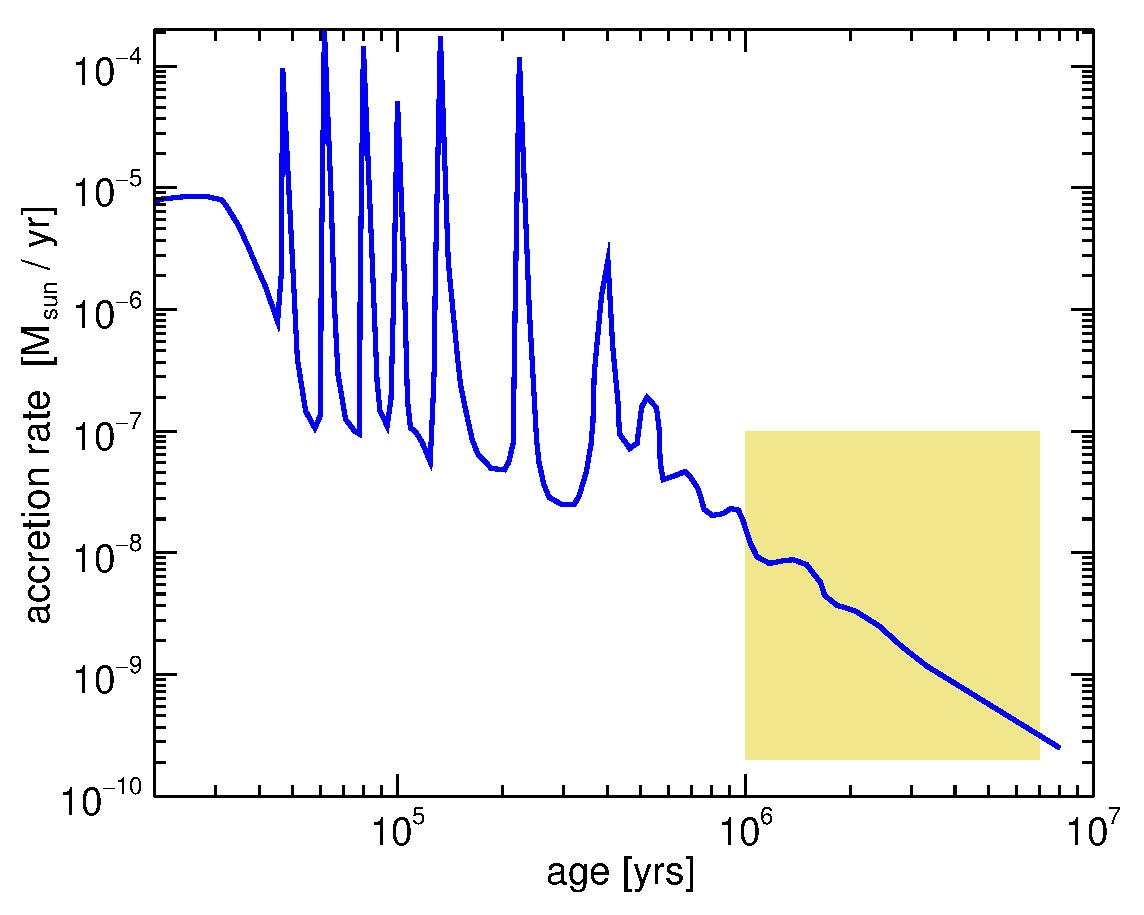
\includegraphics[width=6.3cm,clip=true]{Mdot-hartmann.eps}
\caption{\small \textbf{Left:} Reproduction of Fig.~1 from Hartmann et al.~(2016),
illustrating the main features of disk accretion in YSOs.
\textbf{Right:} Schematic illustration of the temporal evolution of the accretion rate
(adapted from Hartmann 2008). The light-brown shaded area marks the age range
we address in this project.
\label{hartmann.fig}}
\end{figure} %%%%%%%%%%%%%%%%%%%%%%%%%%%%%%%%%%%%%%%%
 %%%%%%%%%%% Figure %%%%%%%%%%




\smallskip

During the following few Myrs, the disk mass decreases, as some part of
the circumstellar matter is accreted onto the star and another fraction
is removed by a disk wind.
As a consequence, the accretion rate also drops and the spectroscopic 
signatures of disk accretion get weaker; 
the object evolves into a so-called    ``\textbf{weak-line T Tauri star}''
(WTTS).
During this evolution, the structure of the accretion disk also changes.
Observational evidence  shows that many of these older disks 
seem to evolve an inner hole in the disk, i.e.~the dust in the inner few AUs of the
circumstellar environment is somehow cleared \citep[e.g.,][]{Alexander14,Koepferl13}.
This typically happens at an age of roughly $ 2 \dots 5$~Myr, and
the result is a so-called \textbf{transition disk} (TD)
\citep[see][]{Owen16}.
\smallskip

In the subsequent evolution, the remaining material in the outer
disk is dispersed by a strong disk wind.
This final disk dispersal process is very rapid ($\sim 10^5$~years)
and proceeds from inside-out \citep{Ercolano14}. As described below in more detail,
the irradiation with ionizing radiation from the central star seems to be
the most important driving mechanism for this disk wind.

\medskip

In the course of this  evolution, the accretion rate generally decreases with time. 
During the very young, protostellar stages,
the accretion process shows strong
 variability on a wide range of timescales, including rare \citep[see][]{HF15}, 
but very strong
bursts of very rapid accretion (FU~Ori bursts), during
which the accretion rates
can be enhanced  by one or more orders of magnitudes for timescales
from months to decades
\citep[see][and the illustration in Fig.~\ref{hartmann.fig}]{Hartmann16}.
%
With increasing age (and correspondingly lower average accretion rates),
however,
the frequency as well as the amplitude of the accretion rate
bursts is strongly decreasing, and at ages of $\ge 1$~Myr (i.e.~in the
TTS stage) the accretion variability is typically less than a factor $\sim 2-3$
\citep[see][]{Venuti14}.




\medskip

Although this description is mainly based on theoretical arguments and
numerical simulations \citep{Ercolano11,Alexander14}, it is well supported and confirmed by an
increasing body of new observational 
data that were collected during the last several years. 
%
In particular, numerous observations have clearly established that
the fraction of YSO with optically thick disks decreases very
quickly with age. The inferred (e-folding) lifetime of these disks
is only about 2--3~Myr, and the fraction of disks in clusters 
with  ages of $> 5$~Myr is very low \citep[e.g.,][]{Hernandez07}. This yields a clearly
established upper limit to the lifetime of protoplanetary disks of
 less than 10 Myr, which provides 
a very important constraint for theories of planet formation
(especially the formation of gas-giants).

\medskip

While the general picture of the accretion process on YSOs is now quite well established,
several observational facets of the accretion and disk evolution processes
are still not well understood and lack a good explanation.
%
One of these open questions concerns the explanation of  the rather wide distribution 
of individual disk lifetimes
around the median lifetime of about 2.5 Myr.
The observational data show that some 15\% of the stars disperse their disks very quickly, within
just about 1 Myr.  On the other hand, a similar fraction of stars manage to keep their
disks even at ages of more than $5-6$~Myr. 
The exact reason for this considerable differences 
in disk lifetimes is not yet well known.

A second important question concerns the explanation of the observed
wide range of individual stellar accretion rates.
Observations of young clusters, where all the stars have a very similar age,
show that for any given stellar mass, the accretion rates show a scatter
of at least two orders of magnitude (see, e.g., Fig.~16 of Venuti et al.~ 2014).
 The reason why stars with the same age and mass display such a wide
range of accretion rates is also not yet clear.



\bigskip


An aspect of fundamental importance in this context is that the disk is not
just a passive ``road'' for the accreted material,
but there is a close interconnection and interaction between
the TTS and its disk.
%
The properties of the disk determine the global accretion rate 
(e.g., via the viscosity) as well 
as the details of how the disk material is
finally deposited onto the stellar surface. This determines
 not only 
how fast the star can gain
mass via accretion, but also influences the temporal evolution of the 
internal stellar structure (and thus influences the luminosity of the protostar)
as well as the evolution of its rotation rate (which is important for 
magnetic dynamo activity). Recent studies also suggest that the
early accretion history impacts the stellar properties even after
several Myr, i.e.~long after the accretion process has ceased \citep[see][]{Baraffe16}.

On the other hand, the
 luminosity of the central star (which results 
partly from the
release of gravitational energy in the accretion shock at the stellar surface) 
determines the irradiation of the disk,
which is a major heating source for the disk and strongly
influences its temperature structure. This also affects the accretion rate in the
disk, which depends strongly on the
 temperature and the
microphysical properties on the disk (e.g., via the viscosity).


As will be described below in more detail, recent results clearly suggest that the
high-energy radiation of the young star, and in particular the X-ray emission,
 plays a very central role in the evolution
and final dispersal of the circumstellar disk
\citep{Ercolano08a,Ercolano08b,Ercolano09,Owen10,Owen11,Owen12}.



%
This intricate interconnection and interaction between the evolution of the star 
(mass growth rate, rotational evolution, magnetic dynamo activity, level
of high-energy radiation)
and the evolution of the disk (time dependence of the accretion rate
and the disk mass-loss rate)
constitutes several feedback loops and is thus 
of fundamental importance for the understanding of the
evolution of YSOs.


\medskip

In recent years,
circumstellar disks evolved into an extremely prominent research topic 
because they are the sites where planets form. 
The properties of the disk around TTS determine the conditions 
under which the planets form and the observational upper limit on the
disk lifetime places very severe constraints for planet formation 
theories.
This highlights the fact that
\textbf{a good understanding of the properties and the evolution of circumstellar disks is also 
highly relevant for our theories about planet formation and early evolution.}


Since the above mentioned (mostly theoretical and numerical) studies
of the star-disk interaction
suggest that stellar X-ray emission is of enormous 
importance for the structure and the evolution of disks, it also
has far-reaching consequences for the planet formation process
\citep{ER15,2013MNRAS.430.1392R}.
%
It is therefore very important to test these models for disk evolution and disk dispersal,
and their predictions they make, with observations.
For this, a solid understanding of the X-ray
emission properties from YSOs is a basic requirement.


\subsection*{b) X-ray emission from YSOs}

Numerous X-ray observations obtained during the last decades have clearly
established that YSOs in all evolutionary stages from
protostars  to  ZAMS stars show highly elevated levels of X-ray  activity
\citep{FM99,PZH96,PZ02,Preibisch_coup_orig,Preibisch11,Preibisch14}.
Typical X-ray luminosities of $\sim$ solar mass YSOs are about $10^{30}\,\rm erg/s$,
i.e.~are up to $\sim 10^4$ times higher than seen in our current Sun.
The temperatures of the X-ray emitting  plasma on young stars
are typically 10 to 20 MK,  i.e.~about ten times higher than in the solar corona.
The X-ray emission of the young stars is therefore considerably harder than the solar
X-ray spectrum, and contains substantial fluxes in the
energy range above 3~keV.

Although the relations between the X-ray activity of young stars and their
stellar / circumstellar parameters were investigated in many star forming regions,
nearly all of these studies suffered from
limited sensitivities and corresponding incomplete X-ray detections.
These problems were finally solved with the
$Chandra$ Orion Ultradeep Project (COUP), a uniquely deep (10-day long)
observation of the Orion Nebula Cluster (ONC)
with $Chandra$/ACIS \citep[for details of the observation and
data analysis see][]{Getman05}.
It is still the deepest and longest X-ray
observation ever made of a young stellar cluster and
produced the most comprehensive dataset ever acquired on the X-ray
emission of young stars \citep{Preibisch_coup_orig}.
Nearly all of the 1616 detected X-ray sources could be
unambiguously identified with optical or near-infrared counterparts.
With a detection limit of
$L_{\rm X,min} \sim 10^{27.3}$~erg/sec for lightly absorbed
sources, X-ray emission from more than 97\% of the
$\sim 600$
optically visible and well characterized late-type
(spectral types F to M) cluster stars
was detected \citep{Preibisch_coup_orig}. 
Since the COUP TTS sample is {\em complete}, 
 the COUP data do not suffer from the
selection effects that plague the less sensitive X-ray studies of
other young clusters,
where a considerable fraction of the lowest mass stars remained undetected.

Two results of fundamental importance for the proposed project 
derived from the COUP data are, that
\begin{enumerate}

\item X-ray luminosity scales to stellar mass as $L_{\rm X} \propto M^{1.4}$ \citep{Preibisch_coup_orig},
and  

\item the X-ray luminosity of TTS is approximately constant for $\ge 10$~Myr \citep{PF05}
 i.e., during the full period of time for which disks usually exist.
\end{enumerate}

The COUP data also confirmed 
that the strong X-ray emission from YSOs  is predominantly originating from
 a hot, magnetically confined plasma in the stellar corona, which is the result of magnetic
dynamo activity \citep{Preibisch_coup_orig}. 
The high X-ray activity levels are thus thought to be ultimately a consequence of
the very fast rotation of the young stars \citep[e.g.,][]{AP12}.

Theoretical arguments suggest that 
the strong X-ray emission of young stars  has far-reaching implications
for the physical structure and processes in their circumstellar environment 
\citep[e.g.,][]{Glassgold05,Wolk05,EG13}, 
the evolution of the disk \citep[e.g.,][]{Ercolano14}, the
formation of planetary systems \citep[e.g.][]{2013MNRAS.430.1392R}, and the evolution of 
the atmospheres of young planets \citep[e.g.,][]{Johnstone15}.
However, detailed observational diagnostics for these suggested influences
 have been hard to come by, so far.
One of these topics is the
question we want to address in this project: How does the X-ray emission
affect the evolution of the protoplanetary accretion disks?




\subsection*{c) Previous observational results on the relation between 
X-ray emission and accretion disks}

About 15 years ago, 
X-ray observations of young stellar clusters provided the first indications that
the X-ray luminosities of young stars seem to depend on the presence
and the properties of accretion disks \citep[e.g.][]{Stelzer01}.
However, no strong conclusions
could initially be drawn due to problems related to small sample sizes, incompleteness of the
 X-ray detected samples, and ambiguities about the disk properties.
%
A fundamental clarification of the tentative relations between X-ray emission and
the properties of accretion disks was finally provided by the COUP data.
COUP showed unambiguously
and in a statistically significant way
that \textbf{the  absolute as well as the fractional X-ray luminosities
of accreting young stars are systematically {\em lower} by a factor of
 $\sim 2-3$ than the corresponding values for  non-accreting stars.}
%

In order to find possible explanations for this surprising result, a more detailed
analysis of the relation between X-ray emission and disk accretion is required.
The best data on accretion rates and accretion luminosities
available at the time of the COUP project 
were those from the study of \citet{Robberto04},  who 
had determined
accretion rates and accretion luminosities for 30
young stars in the Trapezium cluster from Hubble Space Telescope $U$- and $B$-band photometry.
%
The COUP data showed  a weak anti-correlation of the fractional
X-ray luminosity with accretion rate (and also with accretion luminosity).
However,  the statistical significance of this result was low,
because the number of stars for which estimates of the 
accretion rate were available at that time was too small.
Nevertheless, these results were supported by similar findings from
a deep X-ray survey of the Taurus
star forming region, which  also showed   that
the X-ray activity of accreting young stars appears to be somehow suppressed \citep{Briggs07}.
\medskip



Several possible explanations for this  anti-correlation between X-ray activity 
and mass accretion rate were suggested.
One model assumed that changes in the coronal magnetic field
structure by the accretion process could lead to lower X-ray emission
\citep{Romanova04}. This idea was based on the fact that
the pressure of the accreting material may distort the large-scale
stellar magnetic field and
the magnetospheric transfer of material to the star can give rise to
instabilities of the magnetic fields around the inner disk edge.
The presence of accreting material should also lead to higher
densities in (parts of) the magnetosphere; these high densities
could inhibit magnetic heating of the
accreting material to X-ray emitting temperatures.

Another suggestion was that the  accreting material would cool the corona when it
penetrates into active regions and mixes with hot plasma.
If the plasma would be cooled below a few MK,
its very soft X-ray emission would be essentially undetectable for
the CCD X-ray detectors of $Chandra$ and XMM-Newton, and thus the
observed X-ray luminosity of the accreting stars would be lower
than that of non-accretors
\citep[see also][]{Telleschi07}.


Yet another theory suggested that the stripping of the coronal magnetic field 
by the interaction with the disk might reduce the coronal volume and thus the
X-ray emission \citep{Jardine06}.
In stars without a circumstellar disk,
the coronae extend outwards to the radius where the pressure of the
hot coronal gas overcomes the magnetic field,
explaining the observed increase in the X-ray emission measure
with increasing stellar mass.
In stars that are surrounded by a circumstellar accretion disk,
the outer parts of the coronal magnetic field could be stripped
by the interaction with the disk, and this might explain
the observed lower X-ray luminosities of accreting stars.



%%%%%%%%%%% Figure %%%%%%%%%%
\begin{SCfigure} %%%%%%%%%%%%%%%%%%%%%%%%%%%%%%%%%%%%%%%%
\centering
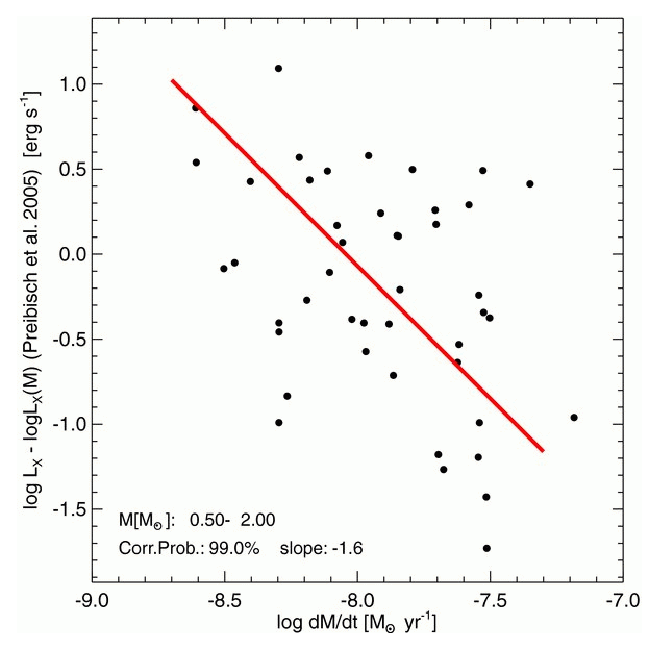
\includegraphics[width=0.45\textwidth]{drake.ps}
\caption{Reproduction of Fig.~3 from Drake, Ercolano, et al.~(2009),
showing the anti-correlation between X-ray luminosity and accretion rate.
\label{drake.fig}}
\end{SCfigure} %%%%%%%%%%%%%%%%%%%%%%%%%%%%%%%%%%%%%%%%
 %%%%%%%%%%% Figure %%%%%%%%%%



\subsection*{d) The new model of photoevaporation-starved accretion}

While the previous models were based on the idea that accretion somehow
suppresses, disrupts or obscures coronal X-ray activity,
\citet{Drake09} developed an alternative
model by suggesting that actually the X-rays modulate the
accretion flow.
They explained this effect with the X-ray heated accretion
disk models of \citet{Ercolano08a,Ercolano08b,Ercolano09} and showed that
photoevaporative mass-loss rates of  disks
are strongly dependent on stellar X-ray luminosity and sufficiently
high to be competitive with accretion rates.
As described in more detail below, the strength of the coronal X-ray emission
determines the accretion rate, and stars with strong X-ray emission should
accrete at lower rates because their disks suffer from higher photo-evaporative
mass-loss rates.
This implies that the stellar X-ray activity controls the evolution of the disk,
and thus should have far-reaching consequences, e.g. on the process
of planet formation and on the disk dissipation timescale.
%

As a first test of this new theory,
\citet{Drake09} compared  X-ray luminosities and accretion rates 
for stars in the Orion Nebula Cluster and found an anti-correlation between
these two quantities (see Fig.~\ref{drake.fig}).
However, these conclusions remained tentative, because they were
based on a rather small sample of
just 44 stars, for which accretion rate estimates
were available at that time.
Because of the fundamental importance of this theory, the relation between X-ray
activity and disk accretion should be tested in much more detail.





\subsection*{e) Disk Dispersal by Photoevaporation}



%%%%%%%%%%% Figure %%%%%%%%%%
\begin{figure} %%%%%%%%%%%%%%%%%%%%%%%%%%%%%%%%%%%%%%%%
\centering
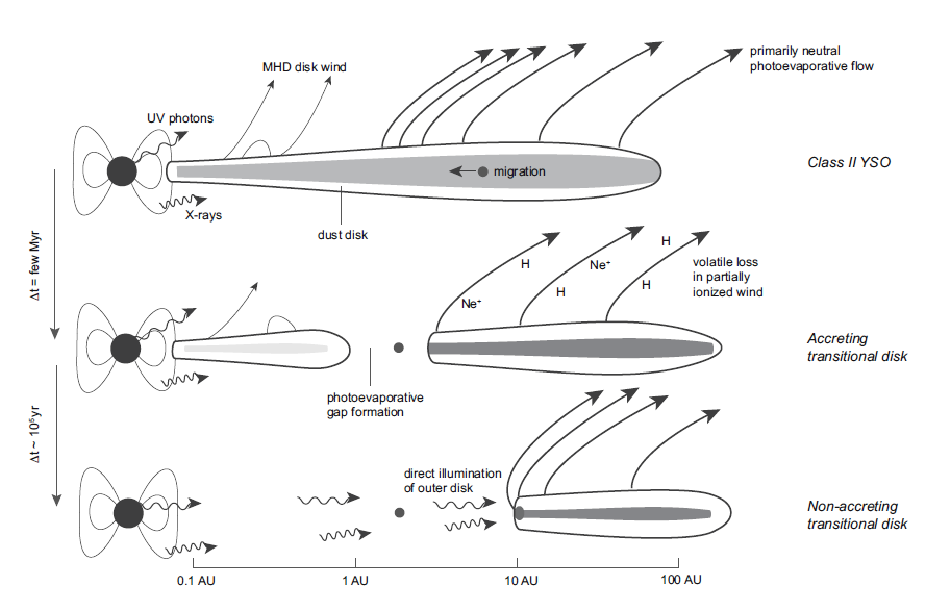
\includegraphics[width=0.95\textwidth]{disk-evolution-alexander.ps}
\caption{Illustration of major steps in the evolution of
a circumstellar accretion disk from the CTTS phase
to the formation of an inner hole and up to the complete
dispersal of the disk \citep[from][]{Alexander14}.
\label{disk-evol-illustration.fig}}
\end{figure} %%%%%%%%%%%%%%%%%%%%%%%%%%%%%%%%%%%%%%%%
 %%%%%%%%%%% Figure %%%%%%%%%%




Theoretical arguments clearly suggest that photoevaporation driven 
by the ionizing radiation from the central young star is the most 
important mean for the dispersal of disks \citep[see][for a recent overview]{Alexander14}.
A simple outline of the physical mechanism is as follows:
The high-energy radiation from the star ionizes the H atoms in the surface layer of the
disk and thereby heats this gas to temperatures of typically
10 000 K. At radii where the corresponding sound speed of the
heated gas ($\sim 10$~km/s) is similar or larger than the escape speed from the
gravitational well (typically a few AU), the hot gas is then essentially unbound; 
it can stream away and escape from the disk in the form of a thermally driven wind.

This mass loss from the outer disk interrupts the supply of material into the
inner parts of the disk, which is still viscously accreting onto the star.
As illustrated in Fig.~\ref{disk-evol-illustration.fig},
this leads to the formation of a hole in the inner regions of the disk.
In the following phases, the outer disk (which is now fully exposed to the
stellar irradiation, because the shielding %by the wind 
from the inner disk does no longer exist)
is finally fully dispersed on rather short timescales.
This sequence of evolutionary steps is illustrated in
Fig.~\ref{disk-evol-illustration.fig}.


Until a few years ago, it was generally assumed that the 
stellar EUV radiation (similar to the chromospheric emission from 
our Sun) is the dominant agent of disk dispersal \citep{Alexander06}.
For the typical EUV fluxes of roughly solar-mass young stars 
($\sim 10^{41}$ photons per second), mass-loss rates of 
$ \dot{\rm M} \sim 3 \times 10^{-10}\,\rm M_\odot/yr$
have been estimated in numerical simulations.
These mass-loss rates are limited by the fact that the stellar EUV photons
can penetrate only to very small values of the gas column density
($N_{\rm H} \sim  10^{18}\,\rm cm^{-2}$), 
because the photo-absorption coefficient for EUV radiation is very high. Therefore,
the EUV radiation  
can ionize only a thin surface layer of the disk, where the 
gas density is quite low. 


Only recently it became clear that stellar X-ray photons 
are probably considerably more efficient in producing 
disk winds \citep{Ercolano08a,Ercolano08b,Ercolano09}.
The fact that the typical fluxes of X-ray photons (roughly
 $10^{39}$ photons per second) are considerably lower than the EUV photon fluxes,
is offset by the much larger 
penetration depth of X-ray photons compared to EUV photons.
As the photo-absorption coefficient for keV photons
is 4 to 5  orders of magnitude lower than for EUV photons, the
X-rays can reach much further down into the deeper layers of the
disk (up to $N_{\rm H} \sim  10^{24}\,\rm cm^{-2}$), 
where the disk densities are much higher. 
Therefore, the X-ray driven 
disk wind starting from these denser regions closer to the
disk midplane can produce much higher mass-loss rates,
around  $ \dot{\rm M} \sim 3 \times 10^{-8}\,\rm M_\odot/yr$
for the typical X-ray fluxes of young stars.


The temporal evolution according to this model depends sensitively
on the flux and the spectrum of the X-ray photons
  and the resulting strength of the
driven disk wind.



%%%%%%%%%%% Figure %%%%%%%%%%
\begin{figure} %%%%%%%%%%%%%%%%%%%%%%%%%%%%%%%%%%%%%%%%
\centering
\includegraphics[width=0.475\textwidth]{model1.ps}\hspace{5mm}
\includegraphics[width=0.475\textwidth]{model2.ps}
\caption{\small Illustration of the temporal evolution of photoevaporative wind
mass loss rate and accretion rate according to the scenario of
X-ray photoevaporation-starved accretion.
The left plot shows the case of a TTS with moderate X-ray luminosity
of $2 \times 10^{29}\,\rm erg/s$. The thick dashed green line shows the
purely viscous accretion rate that would result if there were
no photoevaporation. The dark blue line shows the mass loss rate resulting
from X-ray photoevaporation, and the thick red line the actual accretion rate.
\newline
In the right plot, model curves for the case of a 10 times
higher X-ray luminosity are added.
Comparison of the curves for the accretion rate in both cases
(dark red and orange lines) at the age of 2.5 Myr (solid vertical line)
illustrates the much lower accretion rate
of the high X-ray luminosity case compared to the low  X-ray luminosity case.
\label{PSA_prediction.fig}}
\end{figure} %%%%%%%%%%%%%%%%%%%%%%%%%%%%%%%%%%%%%%%%
 %%%%%%%%%%% Figure %%%%%%%%%%






\subsection*{f) Directions of research in this proposed project}

The model of photoevaporation-starved accretion makes quite specific
predictions on the temporal evolution of the disk accretion rate
as a function of the strength of the X-ray irradiation \citep{Drake09,Owen11}.
As illustrated in Fig.~\ref{PSA_prediction.fig}, the model predicts that
as soon as the viscous accretion rate drops to values comparable to
the wind mass-loss rate due to photoevaporation, an inner disk hole forms
and the accretion rate onto the star will drop strongly within a short period
of time.
This predicts that a higher X-ray luminosity should lead to
an earlier formation of the inner disk hole. At a given time, 
stars with higher levels of X-ray activity should therefore display
lower accretion rates.

\textbf{
An important aim of this project is to test these model predictions with more, and especially
more reliable, observational data.
}
This is very timely now, because during the last few years,
the availability of data required for
reliable accretion rate determinations  has improved very substantially.
This is to a large degree related to
the recent advent of new powerful spectrographs like
X-SHOOTER at the VLT, that combine high spectral resolution
with a very wide wavelength coverage (the entire optical and
near-infrared range, in the case of X-SHOOTER).
Several spectroscopic surveys of young stars in different regions
have been performed in the last few years or are ongoing and provide a wealth
of new, high-quality data, which can be exploited now
\citep[see][]{MT14}.



\subsection{\Tcol Project-related publications}

% Please list your own publications related to the proposed project, 
% adhering to the rules of the DFG guidelines 1.91. In brief, please note: 
% - Up to 10 publications
% - The work must be published or accepted.
% - Publications on astro-ph (arXive, SPIRES or articles with a DOI) count as published. 
% - Any work that is only in the status ``accepted'' MUST be attached to the proposal
%    together with the acceptance letter.
% - All publications in this section CAN be attached to the proposal. Please limit these
%    attachments to a minimum and please note that the reviewers may not read the attachments -
%    the proposal has to speak for itself.
% - The number of allowed publications refers to the sum of the publications listed
%    in ``1.1.1 Articles published or officially accepted by publication outlets...'' and 
%    in ``1.1.2 Other publications''. Publications which only exist on public repositories 
%    belong into the category ``Other Publications''.



\subsubsection{\Tcol 
Articles published or officially accepted by publication outlets with scientific quality assurance;
book publications}

\begin{itemize}

\item
\textbf{Th.~Preibisch}, Y.-C.~Kim, F.~Favata, E.D.~Feigelson, E.~Flaccomio,
K.~Getman, G.~Micela, S.~Sciortino, K.~Stassun, B.~Stelzer, H.~Zinnecker,
2005,
{\em The Origin of T Tauri X-ray Emission: New Insights from
the Chandra Orion Ultradeep Project}, Astrophys.~Journal Supplement
(COUP Special Issue), 160, 401--422
\vspace{-1mm}

\item
\textbf{Th.~Preibisch}, E.D.~Feigelson, 2005,
{\em The evolution of X-ray emission in young stars},
Astrophys.~Journal Supplement (COUP Special Issue), 160, 390--400
\vspace{-1mm}

\item
\textbf{Th.~Preibisch}, S.~Hodgkin, M.~Irwin, J.R.~Lewis, R.R.~King, M.J.~McCaughrean, H.~Zinnecker, L.~Townsley,
P.~Broos, 2011,
{\em Near-Infrared properties of the X-ray emitting young stellar objects in the
Carina Nebula}, Astrophys.~Journal Supplement, 194, 10
\vspace{-1mm}



\item
J.J.~Drake,  \textbf{B.~Ercolano}, E.~Flaccomio, G.~Micela, 2009,
{\em X-ray Photoevaporation-Starved T Tauri Accretion,}
Astrophysical Journal Letters, 699,  L35--L38 
\vspace{-1mm}


\item
\textbf{B.~Ercolano}, 2014,
{\em The dispersal of protoplanetary discs,}
	Astronomische Nachrichten, 335, 549
\vspace{-1mm}


\item
J.E.~Owen, C.J.~Clarke, \textbf{B.~Ercolano}, 2012,
{\em On the theory of disc photoevaporation,}
Monthly Notices of the Royal Astronomical Society, 422, 1880--1901
\vspace{-1mm}


\item
J.E.~Owen, \textbf{B.~Ercolano}, C.J.~Clarke, 2011,
{\em Protoplanetary disc evolution and dispersal: the implications of X-ray photoevaporation,}
Monthly Notices of the Royal Astronomical Society, 412, 13--25 
\vspace{-1mm}



\item
\textbf{B.~Ercolano}, D.~Mayr, J.E.~Owen, G.~Rosotti, C.F.~Manara, 2014,
{\em The $\dot{M}-M_*$ relation of pre-main-sequence stars: a consequence of X-ray driven disc evolution,}
Monthly Notices of the Royal Astronomical Society, 439, 256--263 
\vspace{-1mm}


\item
C.F.~Manara, \textbf{L.~Testi}, 2014,
{\em The imprint of accretion on the UV spectrum of young stellar objects: an X-Shooter view,}
Astrophysics and Space Science, 354, 35-39  

\end{itemize}

\subsubsection{\Tcol Other publications}  \vspace{-1mm}

\subsubsection{\Tcol Patents} \vspace{-3mm}

none \vspace{-3mm}

\section{\Tcol Objectives and work programme}
\renewcommand{\leftmark}{\sc Objectives and work programme}


\subsection{\Tcol Anticipated total duration of the project}

3 years

\subsection{\Tcol Objectives}

In this project, we aim at combining the numerous available deep
X-ray observations of star forming regions in the \textit{Chandra} 
and XMM data
archives with new and reliable measurements of the accretion 
rates of young stars in these regions.
We want to build up a large sample of young stars of different mass
and  age,
for which we then can perform a detailed statistical analysis
of the relation between X-ray activity and accretion in mass- 
and age-stratified stellar sub-samples. 


This was not possible in the past, because accretion rates determinations were only
available for few stars, and even when available, the results were often
plagued by large uncertainties.
%
The main problem with most  previous accretion rate estimates was
 that they were usually
based on color excesses or equivalent-width determinations of single tracer lines
(such as H$\alpha$). The other important parameters, i.e. the  stellar effective
temperature and the extinction, which are needed to convert color excesses or
equivalent-widths to accretion rates, had to be derived from separate observations,
or (more usually) collected from the literature.
This combination of different observational data can easily lead to
substantial uncertainties in the derived accretion rate estimates and the stellar parameters.
%
%
A good example of this is the  study of Orion Nebula Cluster stars by \citet{Robberto04},
who determined
accretion rates for a sample of 40
young stars in the Trapezium cluster from Hubble Space Telescope $U$- and $B$-band photometry.
As the computation of the accretion parameters                          
from the UV excess 
involves numerous assumptions, their values had
considerable uncertainties; for 25\% of their
stars, they found even negative (i.e.~unphysical) values for the accretion luminosities.




The most important advantage of the new high-resolution wide-wavelength range
spectra is that they allow a self-consistent and simultaneous
determination of all the important parameters,  i.e. the
stellar effective temperature, the extinction, and the accretion rate, at the same time and
from one coherent data set.
This results in a far more reliable determination of accretion rates \citep[see][]{MT14}.



The recent study of \citet{Manara13} 
provides a very good illustration of this
fundamental aspect: They investigated two stars in the Orion Nebula Cluster
for which previous data suggested a very strange combination 
of quite old ages ($> 10$~Myr)
and rather high accretion rates (as estimated from the equivalent width
of the H$\alpha$ line).
Manara et al. used  VLT/X-SHOOTER spectra combined
 with an accurate method to re-determine the stellar parameters and the ages of the targets in a 
self-consistent way.
The results of their analysis showed that the earlier
studies had strongly underestimated the extinctions and thus the luminosities
of these two stars. With the new extinction, luminosity, and accretion rate
values derived from X-SHOOTER, these two stars could be shown to be in fact
rather typical accreting young  stars, and not mysterious ``old accretors'' as claimed
before.

\medskip


As described below in more detail, a brief scan through
the available X-ray archive data and matching recent
reliable accretion-rate determinations from the literature
suggests that
it will be possible to construct a sample consisting of several
hundred
young stars.
This number is already much larger than the sample-size of 44
objects, on which the above described previous statistical 
study was based, which yielded strong hints, but no really 
statistically significant proof for an 
anti-correlation between X-ray luminosity and accretion rate.


We also plan to actively enlarge the sample of stars with 
reliable accretion rate measurements by 
%
1) re-analyzing existing X-SHOOTER spectra in the ESO archive
in order to derive accretion rates in a consistent way, and
%
2) performing new X-SHOOTER spectroscopic 
observations of young stars in selected clusters.



{\bf
In this way we will assemble a large, comprehensive, and consistent
database on accretion and X-ray data for YSOs with a wide range of
stellar masses and ages.}
%
With an expected final sample of several hundred objects we can then perform a
 detailed statistical analysis
of the relation between X-ray activity and accretion in mass- and 
age-stratified sub-samples of young stars. 
The results will
provide crucial new
constraints for theoretical models of the X-ray-disk interaction 
by photoevaporation and allow us to
draw conclusions on the expected accretion rate distributions of 
young stars.





\subsection{\Tcol Work programme including proposed research methods}

The work programme consists of three blocks in which high-quality data
on the accretion rates and X-ray luminosities of young stars are collected,
and a final block for the statistical analysis and
comparison to the theoretical models.

In the first block, we want to perform a detailed study
of the $\sim 700$ young stars in the Orion Nebula Cluster, for which
 new and reliable  accretion rate data are now available (part 1a).
%
In this analysis, we will also investigate the possible effects of variability
of the accretion rates as well as the X-ray luminosities
on the correlation between these two parameters (part 1b).
%
Furthermore, using new optical spectroscopic data from recent X-SHOOTER 
and MUSE observations of Orion Nebula Cluster stars,
we want to increase the sample of stars with accretion rate
determinations (part 1c).
\medskip

In the second part of the project we will use the existing X-SHOOTER spectra for
numerous young stars
in various star forming regions to derive new and self-consistent 
measurements of the
stellar parameters and the accretion rates. 
We will determine X-ray luminosities of these stars and then
use these new data,
as well a published results, for a  statistical analysis.
This will allow us to extend the investigation to stars that are
younger or older than the stars in the Orion Nebula Cluster.


\smallskip

In the third part of the project, we plan to obtain new 
X-SHOOTER spectra for selected stars in order to increase the sample
and to optimize the coverage of the parameter space with respect
to stellar age and mass.

\smallskip

In the final part of the project,
all these data will be statistically analyzed and
used to test the theoretical models.


\subsubsection*{Project Part 1: Orion Nebula Cluster}



The first target for this study will be the Orion Nebula Cluster,
for which the COUP data provide the most sensitive and complete
X-ray data set on a sample of about 1000 young stars.

\paragraph*{\hspace*{2mm} 1a: Correlation analysis of the existing X-ray and accretion data}

The first step in the work will be to use the new accretion rates
that have been  determined for $\sim 700$ young stars
in the Orion Nebula Cluster from \citet{Manara12} and correlate them
with the available X-ray data from the COUP project.
%
\citet{Manara12} derived accretion rates from both the U-band excess and the H$\alpha$ luminosity,
after determining empirically both the shape of the typical accretion spectrum across the
Balmer jump and the relation between the accretion luminosity and the  
H$\alpha$ luminosity.
Their tables also report fundamental stellar parameters such as the
effective temperature, extinction, luminosity, radius, and the age. This is
particularly important, since it makes sure that the data on accretion rates are
consistent with the stellar parameters.

This stellar sample will be cross-correlated with the
COUP source table, that lists the X-ray properties of the 1616 X-ray detected objects
in the Orion Nebula Cluster. Due to the large sample size,
this will allow already a much more detailed statistical analysis of the relation between
X-ray activity and accretion properties in mass- and age-stratified samples
than possible before.



\paragraph*{\hspace*{2mm} 1b: Investigating the effects of variability}

The known variability of the X-ray emission as well as the 
temporal variability of the accretion rates is a potential 
complication  for the investigation of the relation between
X-ray emission and accretion, given the fact the X-ray and
accretion rate measurements are usually not obtained simultaneously.
For the case of the ONC, the COUP X-ray observations were performed 
in January 2003, whereas the HST observations, from which the accretion rates
have been determined, were carried out 
between October 2004 and April 2005.
%
We therefore have to take into account the typical amplitudes
of variations on timescales of a few years, and consider
the corresponding possible effects on the correlation analysis.



\smallskip


X-ray luminosities of young stars show typical variations of about
a factor of 2 on timescales of months to years \citep[e.g.][]{Wolk04}.
Stronger variations can, of course,  occur if the star happens to show a
particularly strong X-ray flare during the observation. However,
these flares can easily be recognized by inspection of
the X-ray lightcurve.
%
In the case of the COUP data set, the derived X-ray luminosities
provide an average over more than 10 days, i.e.~more than one
rotation period for almost all of these stars.
Since lightcurves have been analyzed and objects with strong
flares during the observation are known, this information can
be used in the statistical analysis.

\medskip

As described in the introduction and illustrated in Fig.~1,
the variability of the accretion rates in YSOs is strongly dependent
on the age and evolutionary state of the objects.
Very strong variability is expected during the very young, protostellar stages.
%
At the typical ages of our target stars (about 1 to 5 Myr),
accretion rate variability is much more moderate than during the
very young phases.
%
An important quantification of the typical accretion variability of T Tauri stars
was recently
provided by the detailed monitoring study of the young cluster NGC~2264
presented by \citet{Venuti14} and \citet{Venuti15}.
 They found that the variability of the accretion luminosity, as traced
by UV excesses, 
typically amounts to a factor of $\sim 2-3$ on timescales
from weeks to several years. This amplitude of accretion variability
is thus clearly much smaller than the large scatter 
(two to three orders of magnitude)
seen in the distribution of the accretion rates of the cluster stars.
This result shows that the observed wide range of accretions rates
in a young cluster is \textbf{not} primarily due to accretion variability, 
but rather reflects the large range of individual accretion rates of 
the individual stars.
This supports the model we want to test in this project, i.e.~that 
the accretion rate of individual YSOs depends sensitively on the high-energy 
emission of the central  star.

The results from \citet{Venuti14} are consistent with numerous monitoring
studies of YSOs, which also trace the accretion variability as one part
of the total photometric variability of a YSO.
%
%
These studies generally found that the typical
amplitudes of photometric variability of YSOs in the TTS stage
are not more than a few tenths of a magnitude (i.e.~about a factor of two)
on timescales from days to several years.
For the case of the Orion Nebula Cluster, several studies of 
optical variability
on timescales between a few hours and several years
have been performed during the last years
\citep{Herbst02,Stassun06,Stassun07,Parihar09,Rice15} and confirmed
the generally quite moderate levels of variability.
For the large majority of the monitored stars, the observed brightness 
variations were well below about 0.5 magnitudes.

The recent determination of the
frequency of strong accretion rate outbursts for YSOs by \citet{HF15}
also fits into this picture:
 while
the accretion outburst frequency may be as high as
 $10^{-3}\,\mathrm{yr}^{-1}\,\mathrm{star}^{-1}$ for very young
($\le 0.25$~Myr old) protostars, it drops to just about
$3 \times 10^{-6}\,\mathrm{yr}^{-1}\,\mathrm{star}^{-1}$ for
$\ge 1$~Myr old TTS (which are the targets in our project).
This suggests that 
in a sample of $\sim 1000$~TTS,
the likelihood to catch a significant accretion outburst
on at least one star in a 10 year period (i.e.~the upper limit for the
time difference between the X-ray and accretion rate observations)
is just a few percent.


To summarize, these
results are consistent with the assumption that the 
time difference between the
X-ray and accretion rate observations should lead to uncertainties
that are not much larger than about
a factor of $\sim 2-3$ in the accretion rate values for most stars.
While this will increase the scatter in the relations between
X-ray emission and accretion rate, it does not constitute a fundamental problem for
a statistical analysis.
%
The few stars that showed stronger variability in the available
monitoring studies can be excluded or treated separately
in our correlation study.

\medskip


Nevertheless, it cannot be excluded that some objects have
perhaps undergone a larger variation of the accretion luminosity
since the time of the X-ray observation.
In order to identify such possible cases in the Orion sample,
we have recently started a multi-year and multi-color
photometric monitoring project.
%
The aim of this project is to identify stars
that show significant brightness variations indicative of strong accretion rate variability
on timescales from months to years.
%
These observations are performed with our own (LMU) 2m Fraunhofer Telescope 
on Mount Wendelstein. 
The new wide-angle camera WWFI (providing a $0.5^\circ$ field-of-view) 
is ideally suited for this monitoring project, since it allows to cover
the entire cluster, including the full field of the COUP X-ray observation ($17' \times 17'$), in
one exposure. 
Figure \ref{onc-wwfi.fig} shows a first test image of the 
ONC obtained with WWFI with an overlay of the COUP field.
%
A first and preliminary  analysis of these test images shows that more than
450 of the X-ray detected young stars are bright enough (in comparison
to the surrounding nebulosity) to allow a photometric monitoring 
with these data.

We plan to obtain optical images in up to three bands 
about every second week during the season of observability.
Over the 3-year period of the proposed project, this will yield
a comprehensive dataset for a photometric analysis of long-term
variability.
This will thus
allow us to identify objects that show a strong
variation of their brightness on a multi-month to multi-year timescale.
Stars with strong variability on even longer timescales can also be
identified by comparing the photometry from our Wendelstein observations
with older literature data.
%
If any such highly variable objects are identified, they can be excluded
(or treated separately) in the statistical correlation analysis
between X-ray emission and accretion.


%%%%%%%%%%% Figure %%%%%%%%%%
\begin{SCfigure} %%%%%%%%%%%%%%%%%%%%%%%%%%%%%%%%%%%%%%%%
\centering
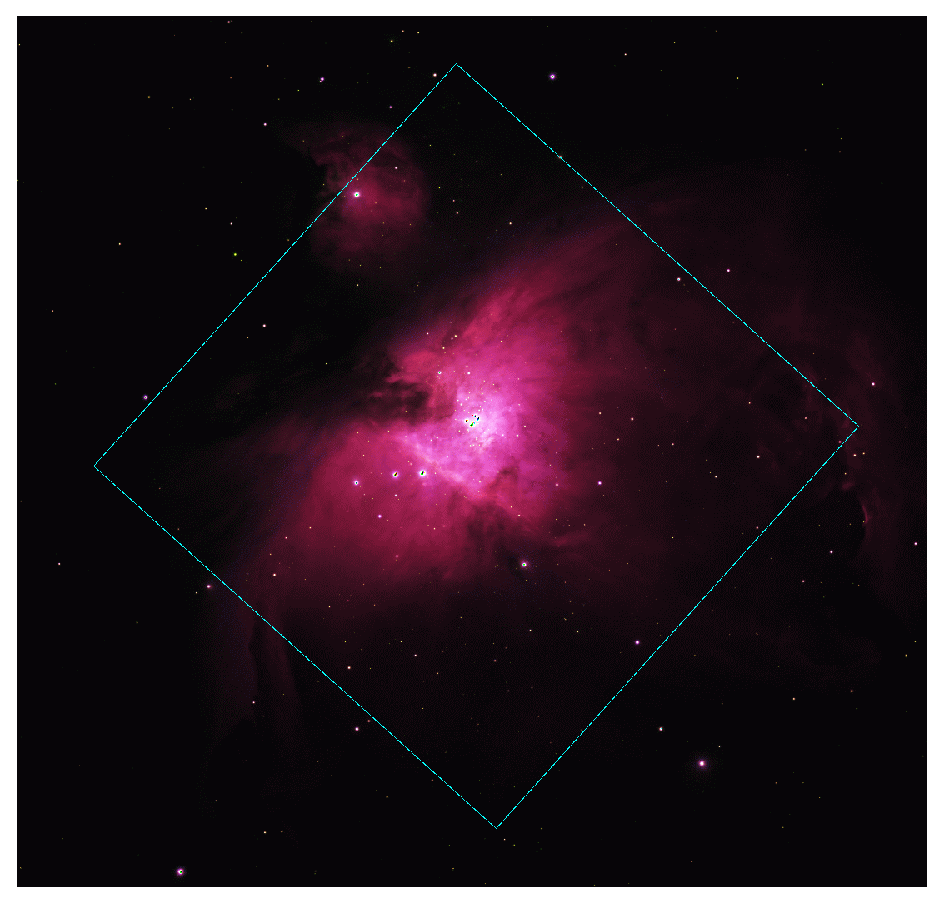
\includegraphics[width=0.5\textwidth]{onc-coupfield-2.ps}
\caption{Optical image of the ONC obtained with the WWFI camera
at our 2m Fraunhofer Telescope on Mount Wendelstein.
The image is a three-color composite of $g$-band (blue), $r$-band
(red), and $i$-band (green) exposures.
The cyan rectangle shows the $17' \times 17'$
field of the COUP X-ray observation.
\label{onc-wwfi.fig}}
\end{SCfigure} %%%%%%%%%%%%%%%%%%%%%%%%%%%%%%%%%%%%%%%%
 %%%%%%%%%%% Figure %%%%%%%%%%




\bigskip

\subsubsection*{Part 1c: New accretion rates for ONC}


The young stars in the Orion Nebula cluster have also been
observed with X-SHOOTER data available ??? 
 
TO BE DETERMINED:  HOW MANY OBSERVED STARS.

We will use these data to derive accretion rates for these stars.
This will allow a detailed comparison with the above mentioned accretion rate
determinations and increase the size of the sample, for which we
can correlate accretion and X-ray data.
\medskip



%%%%%%%%%%% Figure %%%%%%%%%%
\begin{figure} %%%%%%%%%%%%%%%%%%%%%%%%%%%%%%%%%%%%%%%%
\centering
\includegraphics[width=0.45\textwidth]{plot_COUP_758.ps}
\includegraphics[width=0.45\textwidth]{plot_COUP_855.ps}
\caption{
Spectra of two stars (COUP 758 and COUP 855) extracted during our preliminary analysis
of the MUSE data cube of the Orion Nebula.
\label{muse-spectra.fig}}
\end{figure} %%%%%%%%%%%%%%%%%%%%%%%%%%%%%%%%%%%%%%%%
 %%%%%%%%%%% Figure %%%%%%%%%%


Another very interesting spectroscopic dataset was recently
obtained with the 
ESO Multi Unit Spectroscopic Explorer (MUSE), 
an integral-field spectrograph operating in the visible wavelength range
at the ESO 8m Very Large Telescope.
%
The MUSE consortium has released 
data cubes and maps of the Huygens region of the Orion Nebula
published by \citep{Weilbacher15}. %  A\&A 528, A114 
%
These data provide a spatial sampling of $0.2''$ per pixel, 
a spectral resolution of 0.85 \AA \, per pixel, and 
cover the wavelength range 4595 \AA \, to 9366 \AA.
%
We have retrieved and inspected these data, and found that useful
optical spectra can be extracted for at least 359 of the 
COUP X-ray sources.
Two examples of objects with strong emission lines, indicative 
of high accretion rates, are shown in Fig.~\ref{muse-spectra.fig} 

These MUSE spectra can complement the X-SHOOTER data and thus increase 
the number of stars with spectroscopic accretion rate determinations.
Finally, a comparison of MUSE and X-SHOOTER spectra for stars observed
with both instruments can also provide important information 
on time variability of the accretion rates.



\subsubsection*{Part 2: New accretion rates for other star forming regions}

In the second part of the project, we will extend the analysis to young stars in other
star forming regions, for which either reliable accretion rate determinations
or X-SHOOTER spectra are available.
Correlating these data with \textit{Chandra} and XMM X-ray 
observations will provide
further samples of young stars, in which we can investigate the
relation between X-ray luminosity and accretion.
%
This will allow us to extend the parameter space, e.g. by observations
of clusters that are somewhat younger or older than the Orion Nebula Cluster.

Reliable accretion rate determinations are available for the
following regions:
\medskip


{1) NGC~2264:}\\
\citet{Venuti14} determined stellar parameters and accretion rates for about 
750 YSOs in this cluster. Accretion rates were determined from $U$-band excess emission
as well as emission lines. 

This cluster was also extensively studied with \textit{Chandra}: eight deep ACIS-I
observations of the different parts of this region are available in the 
\textit{Chandra} data archive.
\medskip

2) IC 348:\\
\citet{Dahm08} performed a spectroscopic investigation of accretion
diagnostics for 40 near solar mass members of IC~348
and derived accretion luminosities and rates for these stars.

The X-ray properties of these stars are very well known, since IC~348
has been very well observed in X-rays: initially with
ROSAT (Preibisch, Zinnecker, \& Herbig 1996), with
several deep \textit{Chandra} observations (Preibisch \& Zinnecker 2002;
Stelzer, Preibisch. et al.~2012) and also with XMM-NEWTON \citep{PZ04}.
\medskip

Reliable accretion rate determinations and/or X-SHOOTER spectra are also
available for:\smallskip


3) the sigma Ori cluster (accretion rates from U-band photometry from \citet{Rigliaco11};
X-SHOOTER spectra  for 10 stars)
\smallskip

4) the $\rho$ Ophiuchi region (accretion rates for 104 stars from \citet{Natta06};
X-SHOOTER spectra for 17 YSOs from \citet{Manara15})
\smallskip

5) the Lupus region (accretion rates for 36 YSOs from X-SHOOTER spectra by \citet{Alcala14})
\smallskip


6) the Chamaeleon I region (accretion rates from X-SHOOTER spectra by \citet{Manara16})
\smallskip

7) the Upper Scorpius association (X-SHOOTER spectra  for 25 stars)
\smallskip

8) the TW Hya association (X-SHOOTER spectra  for 15 stars)
\smallskip

9) the Taurus region (X-SHOOTER spectra  for $\sim 15$ stars)
\medskip



%
Deep X-ray observations of all these clusters and associations are available in the Chandra and XMM data
archives.  We will retrieve these X-ray data and analyze them in a homogeneous way
using the most recent analysis tools (like ACIS-Extract for the Chandra data) to detect
and characterize X-ray sources. The determination of the X-ray luminosities will be
based on a model fitting analysis of the X-ray spectra with CIAO and XSPEC for sources
with a sufficient number of source counts. For weaker X-ray sources, 
the  X-ray luminosities can be determined from the observed number and energy of the 
detected X-ray photons with the {\tt srcflux} tool in the Chandra analysis software.
Cross-correlating the resulting X-ray source lists with the catalogs of spectroscopically
observed stars will yield the samples for which we can investigate the relations between
X-ray activity and accretion.
\smallskip


In order to extend our database to higher stellar masses, we also plan to analyze 
the available X-ray data for the 91 Herbig AeBe stars (YSOs in the mass range from 
$\approx 2 - 8\,M_\odot$) for which 
accretion rates were determined from X-Shooter spectra in 
the recent study of \citet{Fairlamb16}.


\subsubsection*{Part 3:  New X-SHOOTER observations}

In the course of the project, we also plan to perform new
observations with X-SHOOTER in order to extend the
spectroscopic sample and to optimize the overlap with the X-ray observations.



\subsubsection*{Part 4:  Statistical analysis}


The final aim of the observational part of this project is to get as many and as reliable as 
possible data points to perform
 detailed statistical analysis
of the relation between X-ray activity and accretion in mass- and age-stratified
samples of young stars in different young clusters. This
will provide crucial new
constraints for theoretical models of the X-ray-disk interaction.


The earlier theories (described in Sect.~1c) that tried to explain how
accretion somehow may reduce the X-ray emission, 
could not make testable predictions.
The proposed effects (like changes in the coronal magnetic field structure by the
accreted material, stripping of the coronal magnetic field 
by the interaction with the disk, or a reduced differential rotation in the star
due to magnetospheric coupling) would depend very sensitively on the details
of the interaction. The resulting reduction of the X-ray luminosities could
be quite strong, but also rather weak, and should thus essentially introduce
scatter in the relations between the X-ray properties and accretion properties.

The Drake, Ercolano, et al.~(2009) model, however, makes a rather clear
prediction that the observed accretion rate for stars at a given age
should scale inversely proportional to the X-ray luminosity.
This direct relation between accretion and X-ray luminosity can be tested with
the observational data in different mass and age regimes.








\subsection{\Tcol Data handling}

All required tools for analyzing the X-ray and optical data are available.

\subsection{\Tcol Other information}
% Please use this section for any additional information you feel is
% relevant which has not been provided elsewhere.
\vspace{-2mm}

none
\vspace{-2mm}

\subsection{\Tcol Information on scientific and financial involvement of international cooperation partners}
\vspace{-2mm}

none
\vspace{-2mm}

\section{\Tcol Bibliography}
\vspace{-2mm}

%%%%% Bibliography of all papers cites throughout the proposal %%%%%%%%%%%%%%


%\begin{multicols}{2} 

\begin{thebibliography}{}
{\small

\bibitem[Alcal{\'a} et al.(2014)]{Alcala14} Alcal{\'a}, J.~M., Natta, A., Manara, C.~F., et al.\ 2014, \aap, 561, A2 
\vspace{-2mm}

\bibitem[Alexander \& Preibisch(2012)]{AP12} Alexander, F., \& Preibisch, T.\ 2012, \aap, 539, A64
\vspace{-2mm}

\bibitem[Alexander et al.(2006)]{Alexander06} Alexander, R.~D., Clarke, C.~J., \& Pringle, J.~E.\ 2006, \mnras, 369, 216 
\vspace{-2mm}

\bibitem[Alexander et al.(2014)]{Alexander14} Alexander, R., Pascucci, I., Andrews, S., Armitage, P., \& Cieza, L.\ 2014, Protostars and Planets VI, 475
\vspace{-2mm}

\bibitem[Baraffe et al.(2016)]{Baraffe16} Baraffe, I., Elbakyan, V.~G., Vorobyov, E.~I., \& Chabrier, G.\ 2016, \aap, in press [arXiv:1608.07428]
\vspace{-2mm}

%\bibitem[Bouvier et al.(2007)]{Bouvier07} Bouvier, J., Alencar, S.~H.~P., Boutelier, T., et al.\ 2007, \aap, 463, 1017 

\bibitem[Briggs et al.(2007)]{Briggs07} Briggs, K.~R., G{\"u}del, M., Telleschi, A., et al.\ 2007, \aap, 468, 413 
\vspace{-2mm}

\bibitem[Dahm(2008)]{Dahm08} Dahm, S.~E.\ 2008, \aj, 136, 521-547 
\vspace{-2mm}

\bibitem[Drake et al.(2009)]{Drake09} Drake, J.~J., Ercolano, B., Flaccomio, E., \& Micela, G.\ 2009, \apjl, 699, L35
\vspace{-2mm}

\bibitem[Ercolano(2014)]{Ercolano14} Ercolano, B.\ 2014, Astronomische Nachrichten, 335, 549
%The dispersal of protoplanetary discs
\vspace{-2mm}

\bibitem[Ercolano \& Glassgold(2013)]{EG13} Ercolano, B., \& Glassgold, A.~E.\ 2013, \mnras, 436, 3446 
%X-ray ionization rates in protoplanetary discs
\vspace{-2mm}

\bibitem[Ercolano \& Owen(2016)]{EO16} Ercolano, B., \& Owen, J.~E.\ 2016, \mnras, 460, 3472 
\vspace{-2mm}

\bibitem[Ercolano \& Rosotti(2015)]{ER15} Ercolano, B., \& Rosotti, G.\ 2015, \mnras, 450, 3008 
%The link between disc dispersal by photoevaporation and the semimajor axis distribution of exoplanets
\vspace{-2mm}

\bibitem[Ercolano \& Owen(2010)]{Ercolano10} Ercolano, B., \& Owen, J.~E.\ 2010, \mnras, 406, 1553
%Theoretical spectra of photoevaporating protoplanetary discs: an atlas of atomic and low-ionization emission lines
\vspace{-2mm}

\bibitem[Ercolano et al.(2008a)]{Ercolano08a} Ercolano, B., Young, P.~R., Drake, J.~J., \& Raymond, J.~C.\ 2008a, \apjs, 175, 534-542 
%X-Ray Enabled MOCASSIN: A Three-dimensional Code for Photoionized Media
\vspace{-2mm}

\bibitem[Ercolano et al.(2008b)]{Ercolano08b} Ercolano, B., Drake, J.~J., Raymond, J.~C., \& Clarke, C.~C.\ 2008b, \apj, 688, 398-407 
%X-Ray-Irradiated Protoplanetary Disk Atmospheres. I. Predicted Emission-Line Spectrum and Photoevaporation
\vspace{-2mm}

\bibitem[Ercolano et al.(2009)]{Ercolano09} Ercolano, B., Clarke, C.~J., \& Drake, J.~J.\ 2009, \apj, 699, 1639
%X-Ray Irradiated Protoplanetary Disk Atmospheres. II. Predictions from Models in Hydrostatic Equilibrium
\vspace{-2mm}

\bibitem[Ercolano et al.(2011)]{Ercolano11} Ercolano, B., Bastian, N., Spezzi, L., \& Owen, J.\ 2011, \mnras, 416, 439
%On the lifetime of discs around late-type stars
\vspace{-2mm}

\bibitem[Ercolano et al.(2015)]{Ercolano15} Ercolano, B., Koepferl, C., Owen, J., \& Robitaille, T.\ 2015, \mnras, 452, 3689 
%Far-infrared signatures and inner hole sizes of protoplanetary discs undergoing inside-out dust dispersal
\vspace{-2mm}

\bibitem[Fairlamb et al.(2016)]{Fairlamb16} Fairlamb, J.~R, Oudmaijer, R.~D, Mendigutia, I., et al.\ 2016, 
\mnras, in press [arXiv:1610.09636]
\vspace{-2mm}

\bibitem[Feigelson \& Montmerle(1999)]{FM99} Feigelson, E.~D., \& Montmerle, T.\ 1999, \araa, 37, 363 
\vspace{-2mm}

%\bibitem[Flaherty et al.(2016)]{Flaherty16} Flaherty, K.~M., DeMarchi, L., Muzerolle, J., et al.\ 2016, ApJ, in press [arXiv:1609.09100]
%\vspace{-2mm}


\bibitem[Getman et al.(2005)]{Getman05} Getman, K.~V., Flaccomio, E., Broos, P.~S., et al.\ 2005, \apjs, 160, 319 
\vspace{-2mm}

\bibitem[Glassgold et al.(2005)]{Glassgold05} Glassgold, A.~E., Feigelson, E.~D., Montmerle, T., \& Wolk, S.\ 2005, Chondrites and the Protoplanetary Disk, 341, 165
\vspace{-2mm}

%\bibitem[Gullbring et al.(2000)]{Gullbring00} Gullbring, E., Calvet, N., Muzerolle, J., \& Hartmann, L.\ 2000, \apj, 544, 927 

\bibitem[Hartmann(2008)]{Hartmann08} Hartmann, L.\ 2008, Accretion Processes in Star Formation,  Cambridge University Press
\vspace{-2mm}

\bibitem[Hartmann et al.(2016)]{Hartmann16} Hartmann, L., Herczeg, G., \& Calvet, N.\ 2016, \araa, 54, 135 
\vspace{-2mm}

\bibitem[Herbst et al.(2002)]{Herbst02} Herbst, W., Bailer-Jones, C.~A.~L., Mundt, R., Meisenheimer, K., \& Wackermann, R.\ 2002, \aap, 396, 513 
\vspace{-2mm}

\bibitem[Hern{\'a}ndez et al.(2007)]{Hernandez07} Hern{\'a}ndez, J., Hartmann, L., Megeath, T., et al.\ 2007, \apj, 662, 1067 
\vspace{-2mm}

\bibitem[Hillenbrand \& Findeisen(2015)]{HF15} Hillenbrand, L.~A., \& Findeisen, K.~P.\ 2015, \apj, 808, 68 
\vspace{-2mm}

\bibitem[Jardine et al.(2006)]{Jardine06} Jardine, M., Collier Cameron, A., Donati, J.-F., Gregory, S.~G., \& Wood, K.\ 2006, \mnras, 367, 917
\vspace{-2mm}

\bibitem[Johnstone et al.(2015)]{Johnstone15} Johnstone, C.~P., G{\"u}del, M., St{\"o}kl, A., et al.\ 2015, \apjl, 815, L12
\vspace{-2mm}

\bibitem[Koepferl et al.(2013)]{Koepferl13} Koepferl, C.~M., Ercolano, B., Dale, J., et al.\ 2013, \mnras, 428, 3327
%Disc clearing of young stellar objects: evidence for fast inside-out dispersal
\vspace{-2mm}

\bibitem[Manara et al.(2012)]{Manara12} Manara, C.~F., Robberto, M., Da Rio, N., et al.\ 2012, \apj, 755, 154
\vspace{-2mm}

\bibitem[Manara et al.(2013)]{Manara13} Manara, C.~F., Beccari, G., Da Rio, N., et al.\ 2013, \aap, 558, A114 
\vspace{-2mm}

\bibitem[Manara et al.(2015)]{Manara15} Manara, C.~F., Testi, L., Natta, A., \& Alcal{\'a}, J.~M.\ 2015, \aap, 579, A66
\vspace{-2mm}

\bibitem[Manara et al.(2016)]{Manara16} Manara, C.~F., Fedele, D., Herczeg, G.~J., \& Teixeira, P.~S.\ 2016, \aap, 585, A136 
\vspace{-2mm}


\bibitem[Manara \& Testi(2014)]{MT14} Manara, C.~F., \& Testi, L.\ 2014, \apss, 354, 35 
\vspace{-2mm}

\bibitem[Natta et al.(2006)]{Natta06} Natta, A., Testi, L., \& Randich, S.\ 2006, \aap, 452, 245
\vspace{-2mm}


\bibitem[Owen et al.(2010)]{Owen10} Owen, J.~E., Ercolano, B., Clarke, C.~J., \& Alexander, R.~D.\ 2010, \mnras, 401, 1415
%Radiation-hydrodynamic models of X-ray and EUV photoevaporating protoplanetary discs
\vspace{-2mm}

\bibitem[Owen, Ercolano \& Clarke(2011)]{Owen11} Owen, J.~E., Ercolano, B., \& Clarke, C.~J.\ 2011, \mnras, 412, 13
%Protoplanetary disc evolution and dispersal: the implications of X-ray photoevaporation
\vspace{-2mm}

\bibitem[Owen et al.(2012)]{Owen12} Owen, J.~E., Clarke, C.~J., \& Ercolano, B.\ 2012, \mnras, 422, 1880 
%On the theory of disc photoevaporation
\vspace{-2mm}

\bibitem[Owen(2016)]{Owen16} Owen, J.~E.\ 2016, \pasa, 33, e005 
\vspace{-2mm}

\bibitem[Parihar et al.(2009)]{Parihar09} Parihar, P., Messina, S., Distefano, E., Shantikumar, N.~S., \& Medhi, B.~J.\ 2009, \mnras, 400, 603 
\vspace{-2mm}

\bibitem[Preibisch \& Zinnecker(2002)]{PZ02} Preibisch, T., \& Zinnecker, H.\ 2002, \aj, 123, 1613 
\vspace{-2mm}

\bibitem[Preibisch \& Zinnecker(2004)]{PZ04} Preibisch, T., \& Zinnecker, H.\ 2004, \aap, 422, 1001
\vspace{-2mm}

\bibitem[Preibisch \& Feigelson(2005)]{PF05} Preibisch, T., \& Feigelson, E.~D.\ 2005, \apjs, 160, 390
\vspace{-2mm}

\bibitem[Preibisch, Zinnecker, \& Herbig(1996)]{PZH96} Preibisch, T., Zinnecker, H., \& Herbig, G.~H.\ 1996, \aap, 310, 456
\vspace{-2mm}

\bibitem[Preibisch et al.(2005)]{Preibisch_coup_orig} Preibisch, Th., 
Kim, Y.-C., Favata, F., et al.\ 2005, \apjs, 160, 401
\vspace{-2mm}


\bibitem[Preibisch et al.(2011)]{Preibisch11} Preibisch, T., Hodgkin, S., Irwin, M., et al.\ 2011, \apjs, 194, 10
\vspace{-2mm}

\bibitem[Preibisch et al.(2014)]{Preibisch14} Preibisch, T., Mehlhorn, M., Townsley, L., Broos, P., \& Ratzka, T.\ 2014, \aap, 564, A120
%Gum 31
\vspace{-2mm}

\bibitem[Rice et al.(2015)]{Rice15} Rice, T.~S., Reipurth, B., Wolk, S.~J., Vaz, L.~P., \& Cross, N.~J.~G.\ 2015, \aj, 150, 132 
\vspace{-2mm}

\bibitem[Rigliaco et al.(2011)]{Rigliaco11} Rigliaco, E., Natta, A., Randich, S., Testi, L., \& Biazzo, K.\ 2011, \aap, 525, A47
\vspace{-2mm}

\bibitem[Romanova et al.(2004)]{Romanova04} Romanova, M.~M., Ustyugova, G.~V., Koldoba, A.~V., \& Lovelace, R.~V.~E.\ 2004, \apjl, 616, L151
\vspace{-2mm}

%\bibitem[Romanova et al.(2008)]{Romanova08} Romanova, M.~M., Kulkarni, A.~K., \& Lovelace, R.~V.~E.\ 2008, \apjl, 673, L171 
\bibitem[Robberto et al.(2004)]{Robberto04} Robberto, M., Song, J., Mora Carrillo, G., et al.\ 2004, \apj, 606, 952 
\vspace{-2mm}

\bibitem[Rosotti et al.(2013)]{2013MNRAS.430.1392R} Rosotti, G.~P., Ercolano, B., Owen, J.~E., \& Armitage, P.~J.\ 2013, \mnras, 430, 1392
%The interplay between X-ray photoevaporation and planet formation
\vspace{-2mm}

\bibitem[Sicilia-Aguilar et al.(2010)]{Sicilia-Aguilar10} Sicilia-Aguilar, A., Henning, T., \& Hartmann, L.~W.\ 2010, \apj, 710, 597 
\vspace{-2mm}

\bibitem[Stassun et al.(2006)]{Stassun06} Stassun, K.~G., van den Berg, M., Feigelson, E., \& Flaccomio, E.\ 2006, \apj, 649, 914 
\vspace{-2mm}

\bibitem[Stassun et al.(2007)]{Stassun07} Stassun, K.~G., van den Berg, M., \& Feigelson, E.\ 2007, \apj, 660, 704 
\vspace{-2mm}

\bibitem[Stelzer \& Neuh{\"a}user(2001)]{Stelzer01} Stelzer, B., \& Neuh{\"a}user, R.\ 2001, \aap, 377, 538
\vspace{-2mm}

\bibitem[Stelzer et al.(2012)]{SPA12} Stelzer, B., Preibisch, T., Alexander, F., et al.\ 2012, \aap, 537, A135
\vspace{-2mm}

\bibitem[Telleschi et al.(2007)]{Telleschi07} Telleschi, A., G{\"u}del, M., Briggs, K.~R., Audard, M., \& Palla, F.\ 2007, \aap, 468, 425 
\vspace{-2mm}

\bibitem[Venuti et al.(2014)]{Venuti14} Venuti, L., Bouvier, J., Flaccomio, E., et al.\ 2014, \aap, 570, A82 
\vspace{-2mm}

\bibitem[Venuti et al.(2015)]{Venuti15} Venuti, L., Bouvier, J., Irwin, J., et al.\ 2015, \aap, 581, A66 
\vspace{-2mm}

\bibitem[Weilbacher et al.(2015)]{Weilbacher15} Weilbacher, P.~M., Monreal-Ibero, A., Kollatschny, W., et al.\ 2015, \aap, 582, A114 
\vspace{-2mm}

\bibitem[Wolk et al.(2004)]{Wolk04} Wolk, S.~J., Harnden, F.~R., Jr., Murray, S.~S., et al.\ 2004, \apj, 606, 466
\vspace{-2mm}

\bibitem[Wolk et al.(2005)]{Wolk05} Wolk, S.~J., Harnden, F.~R., Jr., Flaccomio, E., et al.\ 2005, \apjs, 160, 423 
}  % end \scriptsize
\end{thebibliography}
%\end{multicols}




\section{\Tcol Requested modules/funds}
\renewcommand{\leftmark}{\sc  Requested modules/funds}
% Explain each item for each applicant (stating last name, first name).

\subsection{\Tcol Basic Module}

\subsubsection{\Tcol Funding for Staff}
% Please note that funds for your own temporary position (“Eigene Stelleâ€)
% are not to be included here; this belongs to the separate “Module Temporary Positionâ€.

[Text]

\subsubsection{\Tcol Direct Project Costs}

[Text]

\paragraph{\Tcol Equipment up to EUR 10,000, Software and Consumables}

none

\paragraph{\Tcol Travel Expenses}

[Text]

\paragraph{\Tcol Visiting Researchers (excluding Mercator Fellows)}

[Text]

\paragraph{\Tcol Other Costs}

[Text]

\paragraph{\Tcol Project-related publication expenses}

[Text]

\subsubsection{\Tcol Instrumentation}

none

\paragraph{\Tcol Equipment exceeding EUR 10,000} 

none

\paragraph{\Tcol Major Instrumentation exceeding EUR 100,000} 

none

\subsection{\Tcol Module Temporary Position}

[Text]

\subsection{\Tcol Module Replacement Funding}

none

\subsection{\Tcol Module Mercator Fellows}

none

\subsection{\Tcol Module Public Relations Funding}

[Text]

\section{\Tcol Project requirements}
\renewcommand{\leftmark}{\sc Project requirements}

\subsection{\Tcol Employment status information}
% For each applicant, state the last name, first name, and employment
% status (including duration of contract and funding body, if on a
% fixed-term contract).

Thomas Preibisch, Professor at the Ludwig-Maximilians-Universit\"at M\"unchen  (permanent)

Barbara Ercolano, Professor at the Ludwig-Maximilians-Universit\"at M\"unchen  (permanent)

Leonardo Testi, Faculty Member at the European Southern Observatory  (permanent)

\subsection{\Tcol First-time proposal data}
% Only if applicable: Last name, first name of first-time applicant.
\vspace{-2mm}

not applicable
\vspace{-2mm}

\subsection{\Tcol Composition of the project group}
% List only those individuals who will work on the project but will not
% be paid out of the project funds. State each person’s name, academic
% title, employment status, and type of funding.

[Text]

\subsection{\Tcol Cooperation with other researchers}

\subsubsection{\Tcol Planned cooperation on this project}

\paragraph{\Tcol Collaborating researchers for this project within the
  Research Unit}
%Each proposal must be accompanied by a description of how the project
%is integral to the Research Unit, %both in terms of subject matter
%and organisation. This includes a description of the cooperation with
%%others participating within the Research Unit. 

[Text]

\paragraph{\Tcol Collaborating researchers for this project outside of
  the Research Unit}

[Text]

\subsubsection{\Tcol Researchers with whom you have collaborated scientifically within the past three years}
% This information is important for DFG to exclude possible conflicts of interest.
% Please mention not only the names of the cooperation partners but also their institution and city.
% Scientists already mentioned in the previous two subsubsections do not have to be mentioned
% again.

[Text]

\subsection{\Tcol Scientific equipment}
% List larger instruments that will be available to you for the
% project. These may include large computer facilities if computing
% capacity will be needed. 

none

\subsection{\Tcol Project-relevant interests in commercial enterprises}
% Information on connections between the project and the production
% branch of the enterprise.

none


\subsection{\Tcol Additional information}
% If applicable, please list proposals requesting major
% instrumentation and/or those previously submitted to a third party
% here.

none


\end{document}
